\documentclass{article}
\usepackage{fullpage}

\usepackage{epsfig}
\usepackage{amsfonts}
\usepackage{amssymb}
\usepackage{amstext}
\usepackage{amscd}
\usepackage{amsmath}
\usepackage{amsthm}
\usepackage{times}
\usepackage{graphicx}
\usepackage{alltt}
\usepackage{algpseudocode}

\begin{document}

%\thispagestyle{empty}

\noindent
\fbox{
\parbox{\textwidth}{
\begin{Large}
{\bf CS 577: Introduction to Algorithms\hfill Graphs Review Problems}
\end{Large}
}}

\subsection*{Problems}

\begin{enumerate}
%
% Problem 1
%
\item A graph $G = (V, E)$ is \textit{bipartite} if the vertices V can be partitioned into two subsets $L$ and $R$, such that every edge has one vertex in $L$ and the other in $R$.
\begin{enumerate}
\item Prove that every tree is a bipartite graph.
\item Describe and analyze an efficient algorithm that determines whether a given undirected graph is bipartite.
\end{enumerate}

%
% Problem 2
%
\item Let $G$ be a connected graph, and let $T$ be a depth-first spanning tree of $G$ rooted at some node $v$. Prove that if $T$ is also a breadth-first spanning tree of $G$ rooted at $v$, then $G = T$.

%
% Problem 3
%
\item In class we saw that to prove the correctness of Dijkstra's algorithm we need to assert that all edges weights in the graph are nonnegative. In this problem we examine this assumption closely. 
\begin{enumerate}
\item Consider the following algorithm for finding shortest paths in graphs with negative edge weights: add a large constant to each edge weight so that all the weights become positive; then run Dijkstra's algorithm. Is this algorithm correct? Prove your answer.
\item Suppose that the source node $s$ has no incoming edges, and all of the negative weight edges are those that leave $s$ (so, in particular, there are no negative cost cycles). Can Dijkstra's algorithm, started at $s$, fail on such a graph? Prove your answer.
\end{enumerate}

%
% Problem 4
%
\item A \textbf{\textit{number maze}} is an $n \times n$ grid of positive integers. A token starts in the upper-left corner; your goal is to move the token to the lower-right corner. On each turn, you are allowed to move the token up, down, left, or right; the distance you may move the token is determined by the number on its current square. For example, if the token is on a square labeled 3, then you may move the token three steps up, three steps down, three steps left, or three steps right. However, you are never allowed to move the token off the edge of the board.

Describe and analyze an efficient algorithm that either returns the minimum number of moves required to solve a given number maze, or correctly reports that the maze has no solution.
\begin{center}
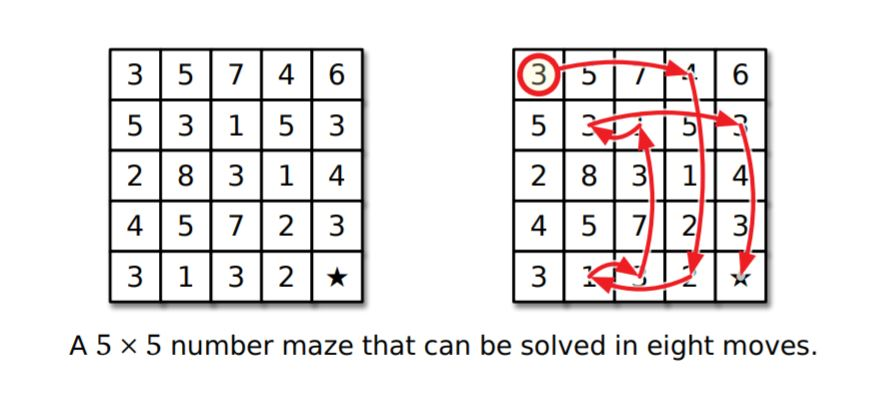
\includegraphics[width=0.7\textwidth]{number_maze.jpg}
\end{center}

%
% Problem 5
%
\item Whenever groups of pigeons gather, they instinctively establish a \textit{pecking order}. For any pair of pigeons, one pigeon always pecks the other. Surprisingly, the overall pecking order can contain cycles--for example, pigeon $A$ pecks pigeon $B$, which pecks pigeon $C$, which pecks pigeon $A$.
\begin{enumerate}
\item Prove that any finite set of pigeons can be arranged in a row from left to right so that every pigeon pecks the pigeon immediately to its left.
\item Suppose you are given a directed graph representing the pecking relationships among a set of $n$ pigeons. The graph contains one vertex per pigeon, and an edge $i \rightarrow j$ if and only if pigeon $i$ pecks pigeon $j$. Describe and analyze an algorithm to compute a pecking order for the pigeons, as guaranteed by part (a).
\end{enumerate}
\end{enumerate}

\end{document}
